\documentclass[10pt]{article}
\usepackage[utf8]{inputenc}
\usepackage{titlesec}

\title{Documentação Biblioteca}
\author{
Victor Miguel de Morais Costa (vmmc2) \\
Zilde Souto Maior Neto (zsmn)
}
\date{}

%%%%%%%%%%%%%%%%%%%%%%%%%%%%%%%%%%%%
\usepackage[colorlinks=true,allcolors=blue]{hyperref}
\usepackage{natbib}
\usepackage{graphicx}
\usepackage[brazilian]{babel}

\usepackage[a4paper,bindingoffset=0.2cm,%
            left=3cm,right=3cm,top=3cm,bottom=3cm,%
            footskip=.65cm]{geometry}
%%%%%%%%%%%%%%%%%%%%%%%%%%%%%%%%%%%%
\begin{document}
\maketitle
%%%%%%%%%%%%%%%%%%%%%%%%%%%%%%%%%%%%

\section{Introdução}
    \begin{itemize}
    \item O presente documento tem como objetivo: descrever, de forma técnica e detalhada, a biblioteca que implementa o protocolo de segurança descrito nas entregas anteriores.
    \end{itemize}

\section{Dependências}
    \begin{itemize}
    \item A biblioteca desenvolvida faz uso de outros pacotes, necessários para auxiliar na implementação de certas funcionalidades da biblioteca. Seu uso se faz necessário principalmente na criptografia presente no protocolo desenvolvido. Os pacotes utilizados foram:
    \begin{enumerate}
        \textbf{\item os}
        \textbf{\item socket}
        \textbf{\item ast}
        \textbf{\item random}
        \textbf{\item collections}
        \textbf{\item base64}
        \textbf{\item Crypto} (Esse pacote específico deve ser instalado por meio do comando: “pip3 install pycryptodome”). A documentação desse pacote em particular pode ser encontrada em: https://pycryptodome.readthedocs.io/en/latest/index.html
    \end{enumerate}
    \end{itemize} 
    
\section{Estrutura}
    \begin{itemize}
    \item A biblioteca desenvolvida foi estruturada de forma que possui 4 classes distintas, que implementam, de forma modularizada, as características do protocolo descritas previamente. 
    \item As classes em questão são: \textbf{bcolors}, \textbf{Socket}, \textbf{Server}, \textbf{Client} e \textbf{Protocol}.
    \item Por questões de organização, a estrutura foi pensada de forma hierárquica, de maneira que existem superclasses e subclasses na biblioteca. A hierarquia mencionada pode ser vista abaixo:
    
    \begin{figure}[ht]
    \centering{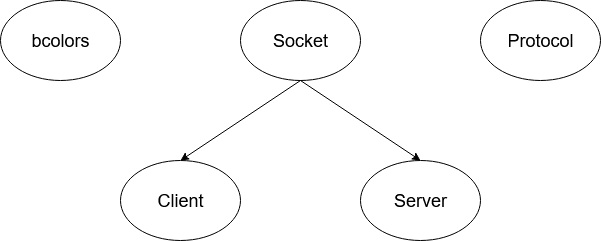
\includegraphics[scale=0.4]{ClassHierarchy.png}}
    \caption{Hierarquia da Biblioteca}
    \label{fig:diagrama}
    \end{figure}
    
    \item Iniciaremos agora a descrição de cada uma das classes, passando por seu objetivo, seus atributos e seus métodos.

    \subsection{\Large bcolors}
        \subsubsection{\large Objetivo}
            \begin{itemize}
            \item A classe tem como objetivo agrupar uma série de códigos de cores e modificadores de
            texto, de forma que as mensagens geradas pela biblioteca possam ser visualizadas mais
            facilmente no terminal pelos usuários.
            \end{itemize}
        \subsubsection{\large Atributos}
            \begin{itemize}
            \item \textbf{bcolors.HEADER:} Atributo responsável por guardar o código responsável por realizar a alteração no texto presente no terminal para o formato cabeçalho/header. \texttt{Tipo: str.} 
            \item \textbf{bcolors.OKBLUE:} Atributo responsável por guardar o código referente à cor Azul. Esse código é utilizado para emitir mensagens de sucesso pela biblioteca. \texttt{Tipo: str.}
            \item \textbf{bcolors.OKCYAN:} Atributo responsável por guardar o código referente à cor Ciano. Esse código é utilizado para emitir mensagens de sucesso pela biblioteca. \texttt{Tipo: str.}
            \item \textbf{bcolors.OKGREEN:} Atributo responsável por guardar o código referente à cor Verde. Esse código é utilizado para emitir mensagens de sucesso pela biblioteca. \texttt{Tipo: str.}
            \item \textbf{bcolors.WARNING:} Atributo responsável por guardar o código utilizado quando a biblioteca emite uma mensagem de aviso/warning. \texttt{Tipo: str.}
            \item \textbf{bcolors.FAIL:} Atributo responsável por guardar o código referente à cor Vermelho. Esse código é utilizado para emitir mensagens de erro/fail pela biblioteca. \texttt{Tipo: str.}
            \item \textbf{bcolors.ENDC:} Atributo responsável por guardar o código que indica que não serão usados outros atributos para modificar a mesma string em questão. Ele sempre é utilizado no final da string. \texttt{Tipo: str.}
            \item \textbf{bcolors.BOLD:} Atributo responsável por guardar o código responsável por realizar a alteração no texto presente no terminal para o formato negrito/bold. \texttt{Tipo: str.} 
            \item \textbf{bcolors.UNDERLINE:} Atributo responsável por guardar o código responsável por realizar a alteração no texto presente no terminal para o formato sublinhado/underline. \texttt{Tipo: str.} 
            \end{itemize}
        \subsubsection{\large Métodos}
            \begin{itemize}
            \item Não há métodos nessa classe.
            \end{itemize}
        
    \subsection{\Large Socket}
        \subsubsection{\large Objetivo}
            \begin{itemize}
            \item A classe tem como objetivo não só criar um socket para que a comunicação entre cliente e servidor ocorra, mas também implementar algumas funcionalidades de criptografia necessárias para o funcionamento adequado do protocolo desenvolvido.
            \end{itemize}
        \subsubsection{\large Atributos}
            \begin{itemize}
            \item \textbf{Socket.socket:} Esse atributo é responsável por guardar o objeto \texttt{socket.socket}, criado no construtor dessa classe e presente no módulo “socket”. \texttt{Tipo: socket.socket.}
            \item \textbf{Socket.address:}  Esse atributo é responsável por armazenar o endereço IP referente ao hospedeiro em questão. \texttt{Tipo: str.} 
            \item \textbf{Socket.port:} Esse atributo é responsável por armazenar o número de porta referente ao socket criado no hospedeiro em questão. \texttt{Tipo: str.}
            \item \textbf{Socket.publicKey:} Esse atributo é responsável por armazenar a chave pública do socket no hospedeiro em questão. \texttt{Tipo: Crypto.PublicKey.RSA.RsaKey.}
            \item \textbf{Socket.privateKey:} Esse atributo é responsável por armazenar a chave privada do socket no hospedeiro em questão. \texttt{Tipo: Crypto.PublicKey.RSA.RsaKey.}
            \end{itemize}
        \subsubsection{\large Métodos}
            \begin{itemize}
            \item \textbf{Socket(address, port):} Esse método é o construtor da classe. O método possui como parâmetros: \underline{address} (O endereço IP do hospedeiro no qual reside o socket. \texttt{Tipo: str.}) e \underline{port} (O número de porta a ser usado pelo socket. \texttt{Tipo: str.}). O método retorna um objeto do \texttt{tipo: protocol.Socket.}
            \item \textbf{Socket.connect():} Esse método é responsável por realizar a conexão de um hospedeiro
            com outro. Uma vez que a forma como a conexão é executada varia de cliente para servidor, essa implementação está vazia e a implementação de fato desse método está presente nas subclasses da classe “Socket”: classe “Client” e classe “Server”. O método não possui nenhum parâmetro e não retorna nada.
            \item \textbf{Socket.generateAssymetricKeys():} Esse método é responsável por gerar as chaves assimétricas (chave privada e chave pública) do socket no hospedeiro em questão. Tanto a chave privada como a chave pública são geradas com o auxílio do pacote “Crypto” mencionado anteriormente. Além disso, é executado automaticamente quando o construtor da classe “Socket” é chamado. O método não possui nenhum parâmetro e não retorna nada.
            \item \textbf{Socket.encryptMessage(message, key, encryptType="assymetric"):} Esse método é responsável por realizar a encriptação de uma mensagem fornecida, dada uma chave e um modo de encriptação. Perceba que o último parâmetro é opcional e, por padrão, será usado o modo de encriptação “assymetric”. O método possui os seguintes parâmetros:
            
            
            \item \textbf{Socket.decryptMessage(message, key, encryptType="assymetric", iv=“‘‘):}
            
            \end{itemize}
        
    \subsection{\Large Server}
        \subsubsection{\large Objetivo}
        \subsubsection{\large Atributos}
        \subsubsection{\large Métodos}
        
    \subsection{\Large Client}
        \subsubsection{\large Objetivo}
        \subsubsection{\large Atributos}
        \subsubsection{\large Métodos}
        
    \subsection{\Large Protocol}
        \subsubsection{\large Objetivo}
        \subsubsection{\large Atributos}
        \subsubsection{\large Métodos}
    \end{itemize}

\section{Conclusão}

\end{document}
